\documentclass[11pt]{article}

\usepackage[T1]{fontenc}
\usepackage[utf8]{inputenc}
\usepackage{lmodern}
\usepackage{microtype}
\usepackage[margin=1in]{geometry}
\usepackage{amsmath,amssymb,mathtools}
\usepackage{booktabs,tabularx,array,longtable}
\usepackage{graphicx}
\usepackage{float}
\usepackage{caption}
\usepackage{xcolor}
\usepackage{enumitem}
\usepackage{fancyhdr}
\usepackage{titlesec}
\usepackage{hyperref}

\definecolor{Ink}{HTML}{26313A}
\definecolor{Muted}{HTML}{68747D}
\definecolor{Blue}{HTML}{2F6B9A}
\definecolor{PaleBlue}{HTML}{EAF1F6}
\definecolor{Gold}{HTML}{C9982F}
\definecolor{Orange}{HTML}{D9773D}
\definecolor{Rule}{HTML}{DCE2E6}

\hypersetup{
  colorlinks=true,
  linkcolor=Blue,
  citecolor=Blue,
  urlcolor=Blue,
  pdftitle={Credit Deterioration Early Warning System},
  pdfsubject={An expository report based on the corrected CreditRisk notebook}
}

\graphicspath{{figures/}}
\captionsetup{font=small,labelfont=bf,labelsep=period}
\setlist[itemize]{leftmargin=1.5em,itemsep=0.35em,topsep=0.4em}
\setlist[enumerate]{leftmargin=1.6em,itemsep=0.35em,topsep=0.4em}
\renewcommand{\arraystretch}{1.16}
\setlength{\parindent}{0pt}
\setlength{\parskip}{0.62em}
\setcounter{tocdepth}{1}

\titleformat{\section}
  {\Large\bfseries\color{Ink}}{\thesection}{0.7em}{}
  [\vspace{0.15em}\color{Rule}\titlerule]
\titleformat{\subsection}
  {\large\bfseries\color{Ink}}{\thesubsection}{0.65em}{}

\pagestyle{fancy}
\fancyhf{}
\setlength{\headheight}{22pt}
\fancyhead[L]{\small\color{Muted}Credit Risk Early Warning System}
\fancyhead[R]{\small\color{Muted}Project Report}
\fancyfoot[C]{\small\color{Muted}\thepage}
\renewcommand{\headrulewidth}{0.4pt}
\renewcommand{\headrule}{\hbox to\headwidth{\color{Rule}\leaders\hrule height \headrulewidth\hfill}}

\newcommand{\pd}{\widehat{\mathrm{PD}}}
\newcommand{\pp}{\text{ percentage points}}
\newcommand{\sourcefile}{\texttt{accepted\_2007\_to\_2018Q4.csv.gz}}
\newcommand{\notebook}{\texttt{CreditRisk\_fixed.ipynb}}

\begin{document}

\hypersetup{pageanchor=false}
\begin{titlepage}
  \centering
  \vspace*{1.2in}
  {\color{Blue}\rule{0.88\textwidth}{2.2pt}}\\[1.1em]
  {\Huge\bfseries\color{Ink}
   Credit Deterioration Early Warning System\par}
  \vspace{0.8em}
  {\Large\color{Muted}From default prediction to risk monitoring and expected loss\par}
  \vspace{1.25em}
  {\color{Gold}\rule{0.42\textwidth}{1.2pt}}\\[2.5em]
  \begin{minipage}{0.80\textwidth}
    \large
    This report explains the current stage of the project. It
    follows the project from data preparation and model design through
    validation, probability calibration, expected loss, and the construction of
    an emerging-risk watchlist. The system is an evolving research prototype,
    and the closing checklist defines the next development cycle.
  \end{minipage}
  \vfill
  {\large Technical project report\par}
  {\color{Muted}10 August 2026\par}
  \vspace{0.55in}
\end{titlepage}
\clearpage
\hypersetup{pageanchor=true}
\pagenumbering{roman}

\section*{Technical summary}
\addcontentsline{toc}{section}{Technical summary}

This project builds a credit risk early warning system that reframes default
prediction as a time-sensitive deterioration problem. Instead of only
classifying loans as default or non-default, the system estimates probability of
default over several time horizons, identifies borrowers whose predicted risk is
accelerating, and translates those probabilities into expected loss. The goal is
an operating view that can place loans into categories such as Healthy,
Watchlist, and High Risk while ultimately explaining the borrower-level drivers
behind each score. The current analysis establishes that foundation and also
makes clear what remains before operational use.

\begin{itemize}
  \item \textbf{The baseline ranking is useful.} A logistic regression trained on
  loans issued through 2014 and evaluated on resolved 2015 loans achieved a
  ROC-AUC of 0.7295 and average precision of 0.4067. Because the test default rate
  was 0.202, average precision was about 2.01 times the random-ranking baseline.

  \item \textbf{Risk bands separate the portfolio clearly, but probabilities are
  too low in the riskiest bands.} For logistic regression, the observed default
  rate increased from 5.5\% in the lowest-risk quintile to 42.3\% in the
  highest-risk quintile. In that highest quintile, the mean predicted probability
  was only 34.4\%, an underprediction of 7.9 percentage points.

  \item \textbf{Gradient boosting adds little discrimination.} Categorical-aware
  histogram gradient boosting increased ROC-AUC from 0.7295 to 0.7314 and average
  precision from 0.4067 to 0.4078. That is a real but operationally small gain.
  Both models remain
  under-calibrated at the high-risk end, suggesting that cohort shift and
  probability calibration matter more than additional nonlinear flexibility.

  \item \textbf{Longer-term loans carry disproportionate risk.} In the resolved
  2015 test cohort, 60-month loans represented 34\% of exposure but 53\% of the
  modelled expected loss under a constant 60\% loss-given-default assumption.
  Their observed default rate was 36.4\%, compared with 14.9\% for 36-month loans.
  This comparison must be read with a selection caveat: only 67.1\% of all 2015
  60-month loans had a resolved terminal status and entered the lifetime test.

  \item \textbf{Horizon-specific models provide the core early-warning view.}
  The 12-, 24-, and 36-month models achieved ROC-AUC values of 0.715, 0.701, and
  0.698. Their ranking lift was strongest at 12 months, while the cumulative
  probability paths supported a small ``emerging risk'' group whose observed
  36-month default rate was 24.0\%, versus 13.4\% under normal monitoring. A new
  discrete-time hazard benchmark keeps unresolved loans and produces monotone
  cumulative probabilities by construction, although its event timing remains
  approximate.

  \item \textbf{The operating layer is now explicit but still scenario-based.}
  A configurable economic review rule combines predicted loss, a 15\% assumed
  intervention effect, a \$50 review cost, and 20\% review capacity. Under those
  illustrative assumptions it selects 84,149 loans and produces \$40.5 million
  of scenario net benefit; this is a decision prototype, not a deployment claim.
\end{itemize}

\textbf{Bottom line.} The current system supports risk ranking, horizon-aware
monitoring, and an initial translation from risk to action. It is not finished:
the scores should not yet be treated as production probabilities for pricing,
capital, or accounting. The next iterations should improve event timing, add
dynamic borrower signals, validate probability and state transitions across
vintages, and replace illustrative operating assumptions with policy-owned inputs.

\tableofcontents
\newpage
\pagenumbering{arabic}

\section{The models rank risk well, but understate its level}

\subsection{The lifetime model provides useful separation}

The first modelling stage uses a simple and interpretable benchmark: logistic
regression. Its task is not to make a hard yes-or-no prediction at a single
threshold. Instead, it assigns every loan a probability of default, which can be
used to rank loans, form risk bands, and estimate expected loss.

\begin{table}[H]
\centering
\caption{Out-of-time performance on resolved loans issued in 2015.}
\label{tab:model-comparison}
\begin{tabular}{lccc}
\toprule
Model & ROC-AUC & Average precision & AP / default-rate baseline \\
\midrule
Logistic regression & 0.7295 & 0.4067 & 2.01$\times$ \\
Categorical-aware boosting & 0.7314 & 0.4078 & 2.02$\times$ \\
\bottomrule
\end{tabular}
\end{table}

ROC-AUC answers a ranking question: if one defaulted loan and one non-defaulted
loan are selected at random, how often does the model give the defaulted loan a
higher score? The value 0.729 means that this ordering is correct about 72.9\% of
the time. Average precision focuses more directly on the rare positive class. A
value of 0.406 against a 0.202 base rate indicates that the score concentrates
defaults near the top of the ranking about twice as effectively as random order.

The model's quintiles make that distinction concrete. The highest-risk fifth of
the test set defaulted at 42.3\%, while the lowest-risk fifth defaulted at 5.5\%.
The ratio is roughly 7.7 to 1. This is meaningful separation for screening and
prioritization.

\subsection{Calibration, rather than ranking, is the immediate weakness}

Figure~\ref{fig:calibration} compares the average predicted probability in each
risk quintile with its observed default rate. Points on the diagonal are perfectly
calibrated. Points above it mean that realized defaults exceeded the model's
prediction.

\begin{figure}[H]
  \centering
  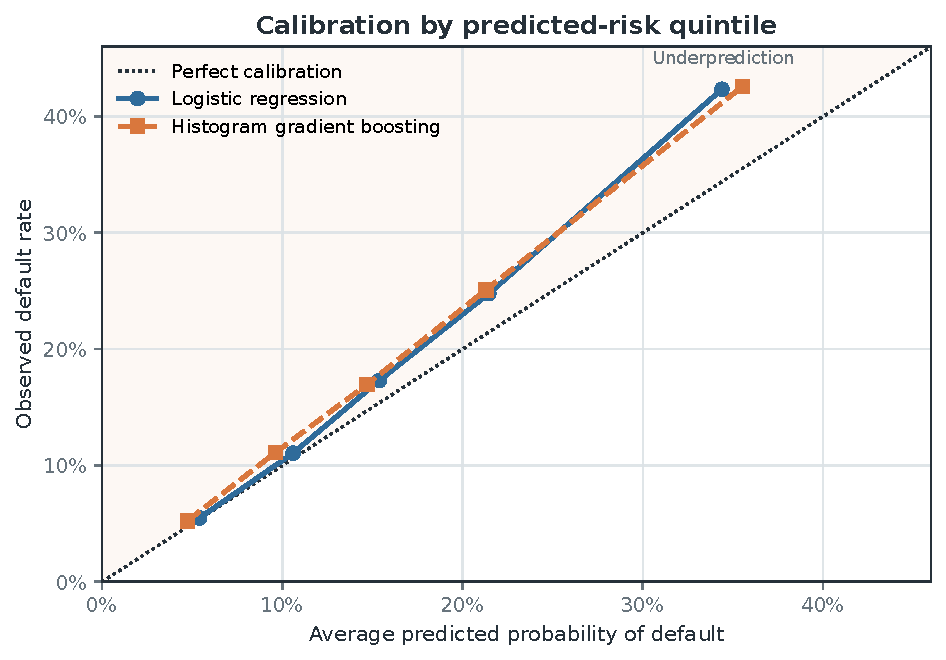
\includegraphics[width=0.84\textwidth]{model_calibration.pdf}
  \caption{Calibration by predicted-risk quintile for the two lifetime models.
  Each point represents approximately one fifth of the 375,546-loan test set.}
  \label{fig:calibration}
\end{figure}

Both curves are close to the diagonal in the lowest-risk bands, then move above it
as risk increases. Logistic regression predicts 34.4\% in its highest band, where
42.3\% is observed. Gradient boosting predicts 35.5\%, where 42.6\% is observed.
The original nonlinear benchmark closes only 0.9 percentage points of the
high-band gap.

This distinction matters. A model may rank borrowers well enough to decide whom to
review first while still producing probabilities that are too low for pricing or
loss estimation. The out-of-time base rate rose from 17.0\% in the training cohort
to 20.2\% in the 2015 test cohort, a shift of 3.16 percentage points. That change
is consistent with the observed underprediction and motivates explicit
recalibration on a more recent, fully observed validation cohort.

The corrected extension implements this temporal calibration design: the model
is fitted through 2013, calibrated on 2014, and evaluated on 2015. Calibration
does not change ranking, but it improves Brier score from 0.1474 to 0.1450 and
moves mean predicted PD from 15.7\% to 17.3\%, closer to the observed 20.2\%.
The remaining gap, especially in the highest decile, shows that recalibration is
helpful but not sufficient.

\subsection{More flexible classification produces only a marginal gain}

Histogram gradient boosting was introduced to capture nonlinear relationships and
interactions that an additive log-odds model may miss. In the corrected comparison,
nominal categories are explicitly marked as categorical rather than treated as a
continuous numeric order. Even so, its improvement is only 0.0019 in ROC-AUC and
0.0010 in average precision. On this feature set, complexity alone does not change
the conclusion.

This result should be interpreted carefully. It suggests that the available
origination variables already carry most of the ranking information exploited by
these two specifications. It does \emph{not} prove that any particular variables
are causal drivers, nor that interactions are unimportant. The notebook does not
include coefficient analysis, permutation importance, SHAP values, or an ablation
study of every individual feature. The new ablation does, however, separate broad
information sources: lender-assigned fields alone reach ROC-AUC 0.710, borrower
and loan fields alone reach 0.716, and the full corrected model reaches 0.729.
This suggests that the system adds information beyond LendingClub's grade and
pricing while still benefiting from those existing underwriting signals.

\section{Term, grade, and cohort composition concentrate risk}

\subsection{Longer terms are riskier, but the resolved-loan sample is selective}

The observed default rate is consistently higher for 60-month loans than for
36-month loans in the resolved-outcome data, as shown in
Figure~\ref{fig:year-term}. The gap is economically important because longer-term
loans also tend to remain exposed for longer.

\begin{figure}[H]
  \centering
  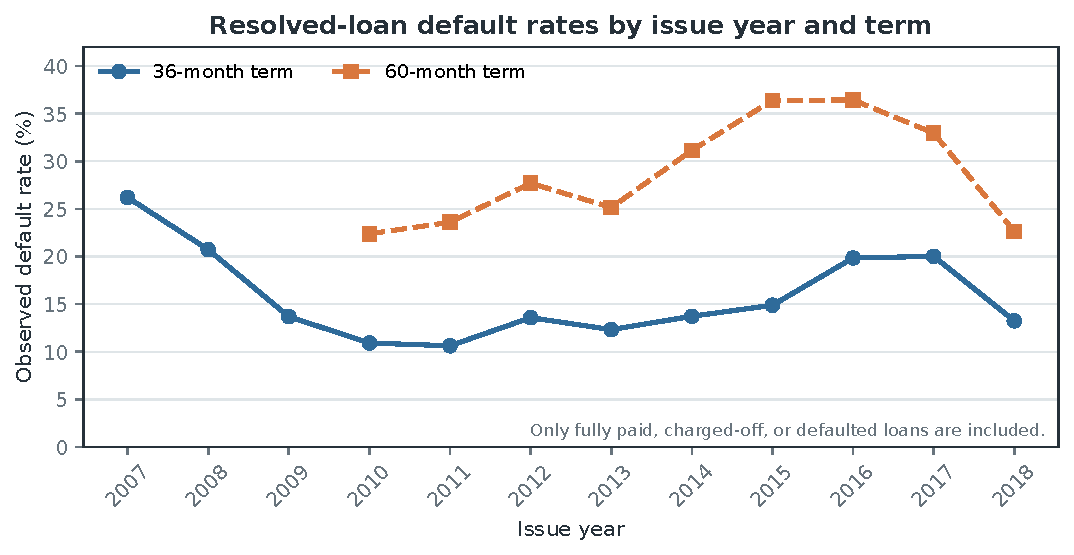
\includegraphics[width=0.94\textwidth]{default_rate_by_year_term.pdf}
  \caption{Resolved-loan default rates by issue year and contractual term. The
  chart describes loans with a terminal good or bad status; it is not a full
  vintage curve for unresolved loans.}
  \label{fig:year-term}
\end{figure}

For 2015, the lifetime test contains 283,026 resolved 36-month loans and 92,520
resolved 60-month loans. Within those samples, the model's ranking is weaker than
its overall ROC-AUC: 0.688 for 36-month loans and 0.669 for 60-month loans. Part of
the aggregate performance therefore comes from separating the higher-risk term
segment from the lower-risk one.

\begin{table}[H]
\centering
\caption{2015 resolved-loan results by term. Expected loss assumes
$\mathrm{LGD}=60\%$ and $\mathrm{EAD}$ equal to original loan amount.}
\label{tab:term-results}
\resizebox{\textwidth}{!}{%
\begin{tabular}{lrrrrrrrr}
\toprule
Term & Loans & Exposure & Predicted PD & Observed default & ROC-AUC & Avg. precision & Expected loss & EL rate \\
\midrule
36 months & 283,026 & \$3.624bn & 13.63\% & 14.89\% & 0.688 & 0.263 & \$285.0m & 7.86\% \\
60 months & 92,520 & \$1.874bn & 29.13\% & 36.39\% & 0.669 & 0.515 & \$322.4m & 17.20\% \\
\bottomrule
\end{tabular}%
}
\end{table}

The exposure comparison is striking: the 60-month segment has about half as much
exposure as the 36-month segment, yet slightly more modelled expected loss. That is
why term belongs in portfolio segmentation and monitoring.

However, this finding is also where sample construction matters most. Among all
421,095 loans issued in 2015, almost every 36-month loan had resolved by the data
cutoff, but 43,227 of the 137,922 60-month loans were still current. Only 67.1\%
of the 60-month vintage entered the terminal-status test. The 36.4\% figure is
therefore a default rate among \emph{resolved} 60-month loans, not among all loans
issued on that term. It should not be used as an unbiased vintage default estimate.

\subsection{Credit grade orders risk, while high grades remain underpredicted}

LendingClub grades produce a strong monotonic risk ordering. Figure~\ref{fig:grade}
shows that observed default increases from 5.5\% in grade A to 54.2\% in grade G.
Under the report's illustrative loss assumptions, expected-loss rate rises from
3.5\% to 25.4\% of original exposure.

\begin{figure}[H]
  \centering
  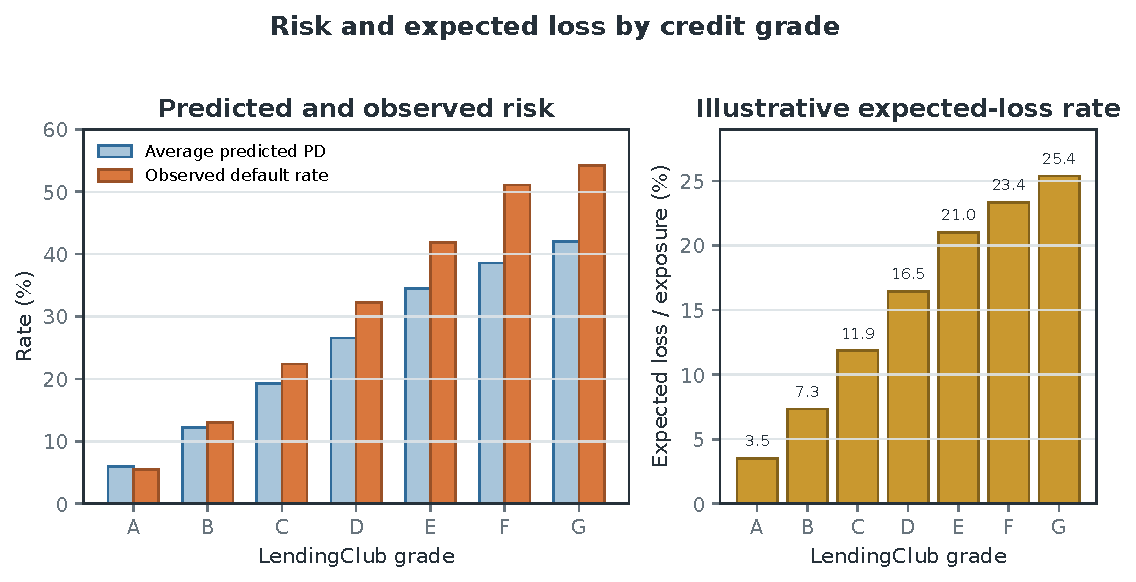
\includegraphics[width=0.98\textwidth]{grade_risk_profile.pdf}
  \caption{Predicted probability, observed default, and illustrative expected-loss
  rate by LendingClub grade for the resolved 2015 test cohort.}
  \label{fig:grade}
\end{figure}

The widening gap between predicted and observed risk in grades D through G echoes
the quintile calibration result. This is operationally significant: an
underestimate in the tail matters more than the same absolute error in a low-risk
band because exposure, review intensity, and loss provisions are often
concentrated there.

The grade result also changes how the model should be described. Grade, sub-grade,
and interest rate are outputs of LendingClub's own underwriting process. Including
them makes the model useful as a portfolio-risk benchmark built on the lender's
origination decisions, but less suitable as an independent underwriting model.
The completed ablation quantifies this distinction: borrower and loan fields alone
produce ROC-AUC 0.716, compared with 0.710 for lender-assigned fields alone and
0.729 for the full corrected model.

\section{Horizon models reveal when risk emerges}

\subsection{Near-term risk is easier to rank from origination information}

The second modelling stage reframes the target. Rather than asking whether a loan
ever ends in default, three models estimate cumulative default risk within 12, 24,
and 36 months. The 12-month model has the highest ROC-AUC and the greatest
average-precision lift relative to its own default-rate baseline.

\begin{table}[H]
\centering
\caption{Out-of-time performance for horizon-specific models on 2015 loans with
adequate outcome information for the relevant horizon.}
\label{tab:horizon-performance}
\begin{tabular}{lrrrrr}
\toprule
Horizon & Test loans & Default rate & ROC-AUC & Avg. precision & AP lift \\
\midrule
12 months & 420,801 & 6.05\% & 0.7150 & 0.1364 & 2.26$\times$ \\
24 months & 420,801 & 13.32\% & 0.7009 & 0.2563 & 1.92$\times$ \\
36 months & 420,748 & 17.37\% & 0.6982 & 0.3166 & 1.82$\times$ \\
\bottomrule
\end{tabular}
\end{table}

Average precision rises with the horizon because the positive class becomes more
common. Its lift over the default-rate baseline moves in the opposite direction,
from 2.26 times at 12 months to 1.82 times at 36 months. This is a more informative
comparison across horizons: origination features distinguish early defaults most
strongly, while later defaults are likely to depend increasingly on borrower
behaviour, macroeconomic conditions, and other post-origination information.

\subsection{Every horizon produces economically distinct risk bands}

Figure~\ref{fig:horizon-bands} compares observed default rates across quintiles
formed separately within each horizon. Within the 36-month model, observed default
rises from 5.3\% in the lowest quintile to 33.3\% in the highest. The same ordering
holds at 12 and 24 months.

\begin{figure}[H]
  \centering
  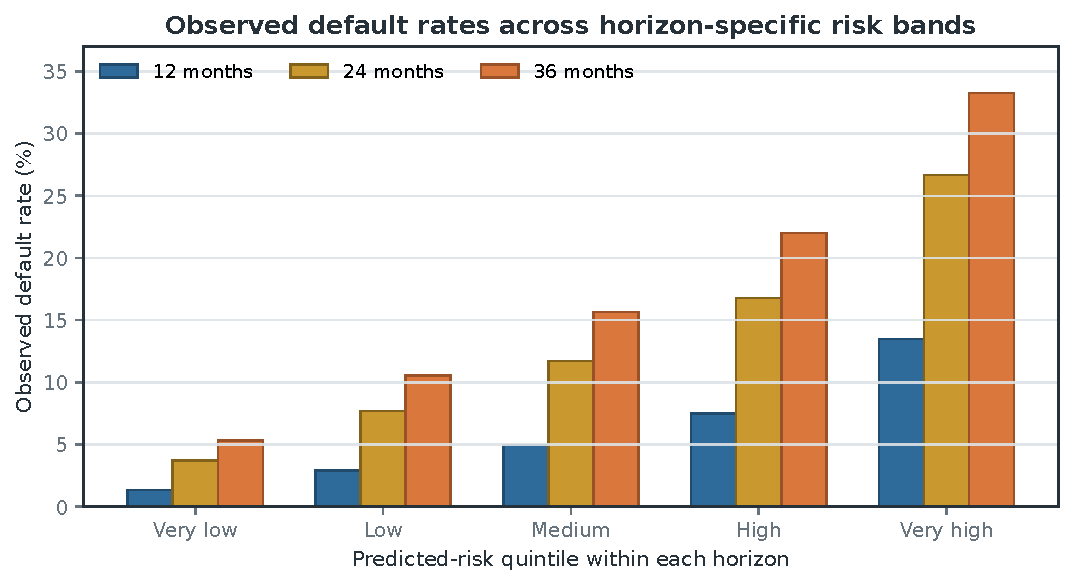
\includegraphics[width=0.94\textwidth]{horizon_risk_bands.pdf}
  \caption{Observed cumulative default rates by horizon-specific predicted-risk
  quintile. Each band contains about 84,150 loans in the common 2015 cohort.}
  \label{fig:horizon-bands}
\end{figure}

This result is more useful than a single lifetime score because it separates two
questions that often call for different actions: which loans are risky now, and
which loans are likely to deteriorate over a longer window? The former can drive
immediate review; the latter can drive monitoring frequency, early-warning rules,
and scenario analysis.

\subsection{Risk acceleration identifies delayed deterioration}

The notebook converts the three independent horizon probabilities into monotone
cumulative paths. It then defines 36-month risk acceleration as adjusted 36-month
PD minus adjusted 12-month PD. Figure~\ref{fig:acceleration} shows that loans with
larger predicted increases also have markedly higher realized 36-month default.

\begin{figure}[H]
  \centering
  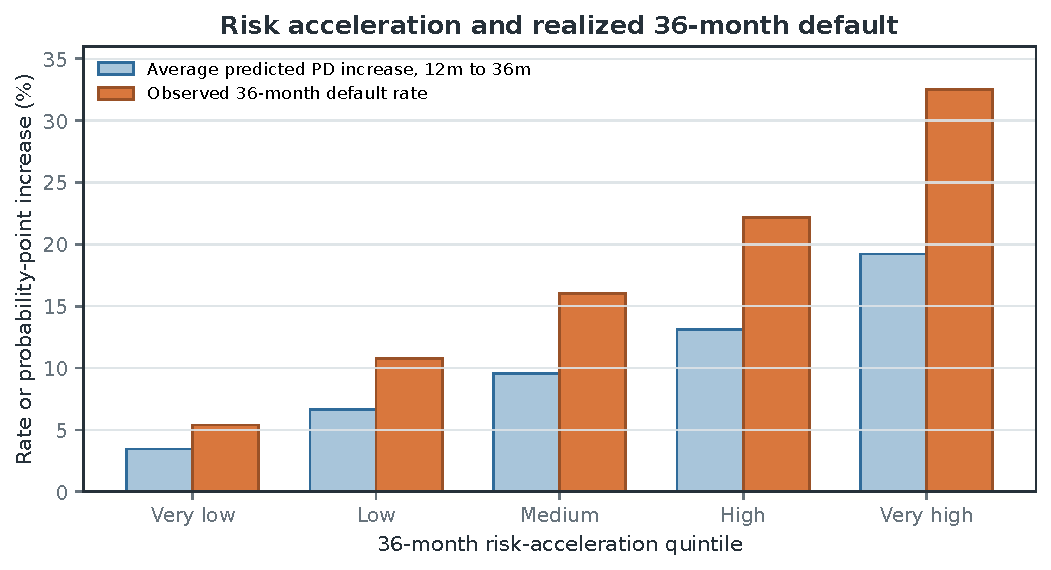
\includegraphics[width=0.93\textwidth]{risk_acceleration.pdf}
  \caption{Average predicted increase from 12-month to 36-month PD and observed
  36-month default rate by acceleration quintile.}
  \label{fig:acceleration}
\end{figure}

The monotonic pattern gives the acceleration concept empirical support. Observed
36-month default rises from 5.4\% in the lowest acceleration quintile to 32.5\%
in the highest. The statistic is still predictive rather than causal: it is a way
of arranging loans by the shape of their modelled risk curve, not evidence that a
particular feature causes later deterioration.

\section{A horizon-aware watchlist turns scores into an operating view}

The final stage groups loans into three monitoring categories:

\begin{itemize}
  \item \textbf{High immediate risk:} 12-month PD is at or above the 80th
  percentile.
  \item \textbf{Emerging risk:} 12-month PD is below the 60th percentile while
  the increase from 12-month to 36-month PD is at or above the 80th percentile.
  \item \textbf{Normal monitoring:} all remaining loans.
\end{itemize}

\begin{table}[H]
\centering
\caption{Watchlist profile in the common 2015 horizon cohort. Expected loss uses
adjusted 36-month PD, a constant 60\% LGD, and original loan amount as EAD.}
\label{tab:watchlist}
\resizebox{\textwidth}{!}{%
\begin{tabular}{lrrrrrrrr}
\toprule
Group & Loans & Share & Avg. 12m PD & Avg. 36m PD & Actual 12m & Actual 36m & Exposure & 36m expected loss \\
\midrule
Emerging risk & 3,132 & 0.74\% & 4.30\% & 21.11\% & 6.67\% & 23.98\% & \$57.2m & \$7.3m \\
High immediate risk & 84,150 & 20.00\% & 10.71\% & 28.40\% & 13.49\% & 32.67\% & \$1.320bn & \$232.4m \\
Normal monitoring & 333,466 & 79.26\% & 3.40\% & 11.89\% & 4.16\% & 13.45\% & \$5.035bn & \$361.4m \\
\bottomrule
\end{tabular}%
}
\end{table}

The emerging-risk group is small, only 0.74\% of the cohort, but its realized
36-month default rate is almost twice the normal-monitoring rate. Its immediate
default rate is much lower than the high-immediate-risk group, which is exactly the
pattern the rule is intended to find: risk that is not extreme at 12 months but
becomes material by 36 months.

The table also illustrates a classic portfolio lesson. Normal monitoring contains
most loans and therefore accounts for about 60\% of total modelled 36-month loss
dollars, even though its per-loan risk is lower. A watchlist is useful for review
and prioritization, but it does not replace portfolio-wide loss estimation.

These three descriptive categories are still defined by percentile rules, so
their meanings can drift as the portfolio changes. The corrected notebook adds a
separate economic overlay that ranks loans by expected loss avoided minus review
cost and selects positive-value cases within a capacity constraint. Under the
illustrative assumptions in the technical summary, the selected 20\% of loans
have a 29.6\% realized 36-month default rate and \$2.005 billion of exposure.
The framework is useful because its assumptions are visible and configurable;
deployment still requires review capacity, intervention effectiveness, cost, and
risk appetite to be estimated and owned by the business.

\section{What was modelled and which loans were eligible}

\subsection{Source population and terminal-status label}

The source file, \sourcefile, contains LendingClub accepted-loan records from 2007
through 2018 Q4. After requiring non-missing loan status and loan amount, the
working source contains 2,260,668 rows. The lifetime-default analysis then keeps
only loans whose terminal status can be interpreted unambiguously as good or bad.

\begin{table}[H]
\centering
\caption{Population flow for the lifetime-default model.}
\label{tab:population-flow}
\begin{tabular}{lrp{0.46\textwidth}}
\toprule
Stage & Loans & Definition \\
\midrule
Source after required fields & 2,260,668 & Non-missing \texttt{loan\_status} and \texttt{loan\_amnt}. \\
Resolved outcome sample & 1,348,099 & Fully paid, charged off, or defaulted, including legacy policy-status variants. \\
Resolved defaults & 269,360 & Charged off, default, or legacy charged-off policy status. \\
Training cohort & 453,809 & Issue year no later than 2014; default rate 17.03\%. \\
Test cohort & 375,546 & Issue year 2015; resolved-outcome default rate 20.19\%. \\
\bottomrule
\end{tabular}
\end{table}

The binary target is
\[
  y_i =
  \begin{cases}
    1, & \text{if loan }i\text{ is charged off or defaulted},\\
    0, & \text{if loan }i\text{ is fully paid}.
  \end{cases}
\]
Loans marked current, late, or in grace period are excluded from this first stage.
That choice gives a clean binary label but creates the resolved-outcome selection
described earlier.

\subsection{Origination features and preprocessing}

The notebook selects 22 source fields, then converts issue date into year and
month. Issue year is used to define the temporal split rather than as an intended
predictor. The modelled information covers five broad areas:

\begin{table}[H]
\centering
\caption{Feature groups used in the project.}
\label{tab:features}
\begin{tabularx}{\textwidth}{@{}p{0.22\textwidth}X@{}}
\toprule
Feature group & Variables \\
\midrule
Loan structure & Loan amount, contractual term, interest rate, installment, and issue month. \\
Lender risk labels & Grade and sub-grade. \\
Borrower capacity & Annual income, employment length, home ownership, verification status, purpose, and debt-to-income ratio. \\
Credit history & Delinquencies in the past two years, FICO range, inquiries in the past six months, open accounts, public records, revolving balance, revolving utilization, and total accounts. \\
Time fields for horizon labels & Issue date and last payment date; these are used to form timing labels and are not intended as outcome predictors. \\
\bottomrule
\end{tabularx}
\end{table}

Missing numeric values are replaced with the training median. Missing categorical
values are replaced with the most frequent training category. Logistic regression
standardizes numeric variables and one-hot encodes categories. Employment length
has the largest missing share at 5.83\%; other selected fields are nearly complete,
with revolving utilization missing in 0.067\% and debt-to-income ratio in 0.028\%.

All preprocessing is held inside a scikit-learn pipeline, so imputation and
encoding are learned on training data and then applied to the test set. This is an
important protection against preprocessing leakage.

\subsection{Eligibility for the horizon targets}

The horizon models require enough follow-up to decide whether a non-default has
survived each horizon. The notebook uses last payment date as an approximate timing
proxy and includes a row if a default appears within the horizon, if at least that
many months are observed, or if the loan was fully paid earlier.

\begin{table}[H]
\centering
\caption{Eligible observations and target rates for horizon-specific labels.}
\label{tab:horizon-populations}
\begin{tabular}{lrrr}
\toprule
Horizon & All eligible rows & Overall default rate & Eligible 2015 test rows \\
\midrule
12 months & 1,901,296 & 6.01\% & 420,801 \\
24 months & 1,592,168 & 13.47\% & 420,801 \\
36 months & 1,422,033 & 18.18\% & 420,748 \\
\bottomrule
\end{tabular}
\end{table}

As the horizon lengthens, fewer loans have adequate observation and more have had
time to default. This changing denominator is why performance and default rates
must be interpreted separately for each horizon.

\section{How the modelling stages were built}

\subsection{Logistic regression as an interpretable baseline}

For a feature vector $x_i$, logistic regression models the probability of default
as
\[
  \pd_i = \Pr(y_i=1\mid x_i)
  = \sigma(\beta_0 + x_i^\top\beta)
  = \frac{1}{1+\exp[-(\beta_0+x_i^\top\beta)]}.
\]
The parameters are fitted by minimizing binary log loss with scikit-learn's
default $L_2$ regularization:
\[
  \mathcal{L}(\beta)
  = -\sum_{i=1}^{n}\left[
      y_i\log(\pd_i) + (1-y_i)\log(1-\pd_i)
    \right]
    + \lambda\lVert\beta\rVert_2^2.
\]

The model is attractive because its output is a probability and its structure is
transparent. Its main restriction is additivity in log-odds. Without explicit
interaction terms, it cannot easily represent a combination whose joint effect is
much stronger than the sum of its parts.

\subsection{Histogram gradient boosting as the nonlinear comparison}

The comparison model builds an additive sequence of shallow decision trees:
\[
  f_M(x) = f_0(x) + \sum_{m=1}^{M}\eta h_m(x),
  \qquad
  \pd(x) = \sigma\!\left(f_M(x)\right),
\]
where $h_m$ is the tree fitted at boosting step $m$ and $\eta=0.05$ is the learning
rate. The notebook uses 200 iterations, at most 31 leaves per tree, at least 100
observations per leaf, $L_2$ regularization of 0.1, and random seed 42.

Numeric variables receive median imputation. Categorical variables receive
most-frequent imputation followed by ordinal encoding, with unseen categories set
to $-1$. The corrected model passes an explicit categorical-feature mask to the
learner, so those codes identify category membership rather than a continuous
ordering. This preserves the computational advantage of the histogram learner
without imposing an artificial scale on purpose, home ownership, and similar
nominal fields.

\subsection{Out-of-time validation}

The main model comparison is trained on loans issued no later than 2014 and tested
on loans issued in 2015. This is more realistic than a random split because it
forces the model to score a later vintage. The calibration extension uses a
stricter three-way split: fitting through 2013, probability calibration on 2014,
and final evaluation on 2015. Both designs reveal temporal drift because the test
cohort has a higher resolved-outcome default rate than the earlier cohorts.

The notebook does not tune hyperparameters through cross-validation. The reported
results are therefore a direct benchmark comparison, not an optimized model
selection exercise. This restraint is useful for interpretation, but uncertainty
around the metric differences is not quantified.

\section{How performance, timing, and expected loss were measured}

\subsection{Discrimination and average precision}

ROC-AUC can be written as the probability of correct pairwise ordering:
\[
  \mathrm{AUC}
  = \Pr(\pd_i > \pd_j \mid y_i=1,\ y_j=0).
\]
Average precision summarizes the precision-recall curve:
\[
  \mathrm{AP} = \sum_{n}(R_n-R_{n-1})P_n,
\]
where $P_n$ and $R_n$ are precision and recall at successive score thresholds.
For a random ranking, expected AP is approximately the positive-class prevalence.
This makes $\mathrm{AP}/\Pr(y=1)$ a useful descriptive lift measure across targets
with different default rates.

\subsection{Calibration by risk band}

For risk band $k$, the report compares the average predicted probability with the
observed default rate:
\[
  \bar p_k = \frac{1}{n_k}\sum_{i\in k}\pd_i,
  \qquad
  \bar y_k = \frac{1}{n_k}\sum_{i\in k}y_i,
  \qquad
  g_k = \bar y_k - \bar p_k.
\]
A positive gap $g_k$ means that the model underpredicts default in that band. This
banded check is easy to communicate, although a production validation should also
report Brier score, calibration intercept and slope, confidence intervals, and
calibration within material subgroups.

\subsection{Horizon labels and monotone probability paths}

Let $m_i$ denote the approximate number of months from issue date to last payment
date. For horizon $h\in\{12,24,36\}$, the target is
\[
  y_i^{(h)} =
  \mathbb{1}\{\text{eventual default}_i=1\ \text{and}\ m_i\le h\}.
\]
An observation is considered valid for horizon $h$ when
\[
  V_i^{(h)} =
  \mathbb{1}\{y_i^{(h)}=1\ \text{or}\ m_i\ge h\
  \text{ or fully paid}_i=1\}.
\]
This rule removes non-defaults with insufficient follow-up unless they fully paid
early. It is a pragmatic censoring rule, but it is not a formal survival model.

Because the three classifiers are fitted independently, their cumulative
probabilities can occasionally violate monotonicity. The notebook applies
\[
  \widetilde p_{12}=p_{12},\qquad
  \widetilde p_{24}=\max(p_{12},p_{24}),\qquad
  \widetilde p_{36}=\max(p_{12},p_{24},p_{36}).
\]
Violations are rare: $p_{24}<p_{12}$ for 0.018\% of the common 2015 cohort and
$p_{36}<p_{24}$ for 0.576\%. The 36-month acceleration statistic is then
\[
  \Delta_i^{36} = \widetilde p_{36,i}-\widetilde p_{12,i}.
\]

The corrected extension also fits a discrete-time hazard benchmark over successive
12-month intervals. If $q_{i,t}$ is the conditional default probability in
interval $t$ for a loan still at risk, cumulative probability is
\[
  \Pr(T_i\le h)=1-\prod_{t\le h}(1-q_{i,t}).
\]
This construction makes cumulative PD monotone without post-processing and keeps
unresolved loans until censoring. The benchmark is trained through 2013,
calibrated on 2014 interval hazards, and evaluated on the common 2015 cohort. Its
12-, 24-, and 36-month ROC-AUC values are 0.676, 0.668, and 0.666; the lower
ranking performance is the cost of a more realistic, but still approximate,
event-time formulation and provides a useful sensitivity check rather than a new
champion model.

\subsection{Expected loss translation}

The project converts probability into an illustrative credit-loss measure using
the standard identity
\[
  \mathrm{EL}_i = \mathrm{PD}_i\times\mathrm{LGD}_i\times\mathrm{EAD}_i.
\]
It assumes a constant $\mathrm{LGD}=60\%$ and sets exposure at default equal to
the original loan amount. For the resolved 2015 lifetime cohort, this gives
\$607.3 million of modelled expected loss on \$5.499 billion of original exposure,
or 11.05\%.

This translation is valuable because it puts model output in monetary terms. It
is also deliberately simplified. Actual EAD changes with amortization and
prepayment; LGD varies with recoveries, collateral, costs, and time; and a full
accounting or capital calculation would incorporate discounting, scenario weights,
and policy definitions.

\section{What the results do not yet establish}

The project is directionally strong, but several limitations materially affect
how its numbers should be used.

\begin{enumerate}
  \item \textbf{Resolved-outcome selection is the main limitation of the lifetime
  model.} Current and delinquent loans are excluded. This is especially important
  for 60-month loans issued in 2015, only 67.1\% of which have a terminal status in
  the source snapshot. The resulting default rates are not unbiased vintage rates.

  \item \textbf{Default timing is approximate.} The horizon labels use
  \texttt{last\_pymnt\_d}, not a clean charge-off or legal default date. Last payment
  may precede the actual default event, so the models should be described as
  approximate early-warning models.

  \item \textbf{Calibration changes over time and by segment.} The later test
  vintage has a higher base rate, and underprediction is strongest in high-risk,
  long-term, and weak-grade groups. Any use of PD in pricing or expected loss needs
  a recent calibration sample and segment-level checks.

  \item \textbf{Some predictors embed the lender's existing risk assessment.}
  Grade, sub-grade, and interest rate are assigned through LendingClub's
  underwriting. Their inclusion is reasonable for portfolio monitoring, but it
  can overstate the model's independent underwriting contribution. The completed
  ablation shows that borrower and loan fields alone retain useful discrimination
  (ROC-AUC 0.716), while the full model remains stronger (0.729).

  \item \textbf{Model interpretability has not yet been demonstrated empirically.}
  Logistic regression is structurally interpretable, but the notebook does not
  report coefficients or stability. Grade, sub-grade, and interest rate are also
  highly related, so individual coefficients may be unstable even when prediction
  is sound.

  \item \textbf{The corrected categorical treatment is only one robustness
  check.} The updated histogram model marks encoded nominal features as
  categorical. Alternative learners and encodings should still be compared under
  the same rolling temporal validation design.

  \item \textbf{Metric uncertainty is not quantified.} The comparison uses one
  out-of-time year and reports point estimates without bootstrap confidence
  intervals, vintage-by-vintage backtests, or statistical tests of the small model
  difference.

  \item \textbf{The event-time benchmark remains approximate.} The new
  discrete-time hazard model handles censoring and produces monotone cumulative PD,
  but it still uses last payment as a default-time proxy and treats prepayment as a
  competing event censored at payoff. A validated competing-risks design is still
  needed.

  \item \textbf{Expected loss is illustrative.} Constant LGD and original loan
  amount as EAD are transparent assumptions, not validated recovery and exposure
  models. The results are not IFRS 9, CECL, regulatory-capital, or pricing estimates.

  \item \textbf{External validity is limited by data vintage.} The file ends in
  2018 Q4. Product policy, borrower mix, servicing, and economic conditions may
  differ materially in a current portfolio.
\end{enumerate}

The raw population counts, status definitions, temporal cohort sizes, and horizon
label rates in the notebook were independently reproduced from the supplied source
file. Model-performance values in this report come from the corrected notebook's
stored outputs. That notebook was executed end to end in a fresh kernel: all 72
code cells completed and no error outputs remained.

\section{Working checklist for the next iteration}

The project is unfinished. The following checklist keeps future work anchored to
the early-warning objective rather than to model complexity for its own sake. The
phases are ordered deliberately: later modelling and operating decisions depend
on the data and event definitions established first.

\subsection*{Phase 1: Establish the data and target foundation}

\begin{itemize}[label=$\square$,leftmargin=2em]
  \item \textbf{Audit the available post-origination data.} Confirm whether monthly
  payment history, days past due, outstanding balance, utilization, bureau updates,
  hardship events, recoveries, and relevant macroeconomic series are available.
  Produce a data dictionary, coverage table, and explicit gap list before choosing
  a dynamic model.

  \item \textbf{Build a leakage-safe loan-month panel.} Create one observation per
  loan per reporting month, preserve only information known at that date, and add
  automated checks for duplicate periods, impossible dates, outcome leakage, and
  inconsistent balances. This panel becomes the canonical dataset for subsequent
  deterioration modelling.

  \item \textbf{Define deterioration and the event clock.} Agree on operational
  definitions for delinquency migration, material PD increase, Watchlist entry,
  High Risk entry, default, cure, prepayment, and exit. Replace last payment with
  the best available event dates and state how competing events will be handled.
\end{itemize}

\subsection*{Phase 2: Develop a genuinely dynamic risk model}

\begin{itemize}[label=$\square$,leftmargin=2em]
  \item \textbf{Create simple behavioural benchmarks first.} Compare the current
  origination model with transparent additions such as recent delinquency status,
  missed-payment counts, payment-to-installment ratio, balance trend, and utilization
  change. Require each added signal to improve out-of-time warning performance.

  \item \textbf{Fit a monthly event-time model.} Estimate conditional 3-, 6-, and
  12-month default risk with a discrete-time hazard or competing-risks model using
  time-varying features. Compare it with the existing horizon classifiers on the
  same loan-month cohorts and cutoffs.

  \item \textbf{Model risk-state transitions.} Estimate movement among Healthy,
  Watchlist, High Risk, Default, Cure, and Exit. Report transition matrices, state
  persistence, and time from first warning to default rather than evaluating only
  terminal classification.
\end{itemize}

\subsection*{Phase 3: Turn scores into stable and explainable alerts}

\begin{itemize}[label=$\square$,leftmargin=2em]
  \item \textbf{Set state rules with persistence and hysteresis.} Define entry,
  escalation, cure, and exit thresholds using calibrated absolute PD, change in PD,
  and severe-event overrides. Require persistence where appropriate so small score
  movements do not repeatedly move an account between states.

  \item \textbf{Measure whether warnings arrive early enough.} Report the share of
  defaults and loss exposure identified 3, 6, and 12 months in advance, median alert
  lead time, precision and recall at review capacity, false alerts, and average time
  spent on the Watchlist.

  \item \textbf{Explain each alert at borrower level.} Show current PD, change from
  the previous observation, horizon of concern, exposure, expected loss, recent
  behavioural events, and a small set of stable reason codes. Validate that the
  explanations remain consistent under correlated predictors.
\end{itemize}

\subsection*{Phase 4: Validate decisions and prepare for controlled use}

\begin{itemize}[label=$\square$,leftmargin=2em]
  \item \textbf{Run rolling temporal and segment backtests.} Repeat
  fit--calibrate--test splits over multiple vintages. Track discrimination,
  calibration, loss capture, warning lead time, and state stability with confidence
  intervals by term, grade, and material borrower segment.

  \item \textbf{Develop realistic LGD and EAD components.} Estimate recoveries,
  collection costs, outstanding exposure, amortization, and prepayment so that the
  economic layer reflects loss at the warning horizon rather than original balance
  and constant severity.

  \item \textbf{Validate intervention economics.} Replace the illustrative 15\%
  effectiveness, \$50 review cost, and 20\% capacity with policy-owned estimates.
  Where possible, use a retrospective comparison or controlled pilot to test which
  actions reduce loss, for which accounts, and at what cost.

  \item \textbf{Define monitoring and governance before deployment.} Assign owners
  for data quality, model changes, thresholds, overrides, and alert outcomes. Set
  review triggers for drift, calibration failure, subgroup deterioration, capacity
  breaches, and realized loss, and document the conditions for rollback or model
  retirement.
\end{itemize}

\section{Questions worth answering next}

\begin{itemize}
  \item How stable is the borrower-and-loan-only model's discrimination after
  removing LendingClub grade, sub-grade, and interest rate across rolling
  vintages and borrower segments?
  \item Does the 2014 calibration improve later vintages and high-risk segments,
  or will calibration require a rolling or segment-specific design?
  \item Which features distinguish emerging-risk loans from loans that are risky
  immediately, after controlling for term and grade?
  \item How stable are the watchlist shares and default rates across issue months,
  vintages, and macroeconomic regimes?
  \item What review threshold maximizes expected loss avoided after review cost,
  false positives, and operational capacity are included?
  \item How much do realistic amortizing EAD and segment-specific LGD change the
  apparent concentration of loss by term, grade, and watchlist group?
\end{itemize}

\appendix
\section{Detailed result tables}

\begin{table}[H]
\centering
\caption{Logistic-regression calibration by risk quintile.}
\label{tab:lr-calibration}
\begin{tabular}{lrrrr}
\toprule
Risk band & Loans & Mean predicted PD & Observed default & Gap \\
\midrule
Very low & 75,110 & 5.40\% & 5.49\% & 0.08 pp \\
Low & 75,109 & 10.60\% & 11.05\% & 0.45 pp \\
Medium & 75,109 & 15.38\% & 17.30\% & 1.92 pp \\
High & 75,109 & 21.46\% & 24.77\% & 3.31 pp \\
Very high & 75,109 & 34.39\% & 42.32\% & 7.93 pp \\
\bottomrule
\end{tabular}
\end{table}

\begin{table}[H]
\centering
\caption{Histogram-gradient-boosting calibration by risk quintile.}
\label{tab:gb-calibration}
\begin{tabular}{lrrrr}
\toprule
Risk band & Loans & Mean predicted PD & Observed default & Gap \\
\midrule
Very low & 75,110 & 4.74\% & 5.24\% & 0.50 pp \\
Low & 75,109 & 9.61\% & 11.09\% & 1.48 pp \\
Medium & 75,109 & 14.70\% & 16.95\% & 2.26 pp \\
High & 75,109 & 21.30\% & 25.08\% & 3.78 pp \\
Very high & 75,109 & 35.52\% & 42.56\% & 7.03 pp \\
\bottomrule
\end{tabular}
\end{table}

\section{Reproducibility note}

The report is based on the current corrected notebook \notebook\ and the local
LendingClub data extract \sourcefile. Figures in this document are redrawn from
the notebook's executed numeric outputs so that the LaTeX source remains portable
and the charts remain sharp when printed. The corrected notebook is the companion
computational artifact for model fitting and row-level analysis; the original
\texttt{CreditRisk.ipynb} remains unchanged.

\end{document}
